\chapter{Normalisation}

% Preprocessing techniques are essential for enhancing signal clarity and improving the accuracy of subsequent analyses. These techniques aim to mitigate unwanted artefacts and noise that can obscure meaningful information within the signal. Among the numerous preprocessing methods developed, here we focus on two specific techniques: detrending and denoising. 

% \begin{researchquestion}
% How effective are preprocessing steps such as normalisation, detrending, and denoising in improving the clarity of underwater acoustic signal recordings?
% \end{researchquestion}

Normalisation is considered a fundamental step in preprocessing spectrograms for machine learning tasks. Its primary purpose is to standardise input data in order to reduce variability in amplitude scales and improve model training stability. By ensuring that all inputs share similar statistical properties, normalisation enhances convergence and reduces the risk of numerical instability. This chapter aims to quantify the benefits of normalisation for use with underwater acoustic datasets such as DeepShip.

\section{Introduction}

The primary motivation for normalisation is to standardise the input data to avoid biases caused by differences in feature magnitudes. Take the following example as illustration: consider two input features $x_1$ and $x_2$ with ranges $x_1 \in [0, 1000]$ and $x_2 \in [0, 1]$ and corresponding weights $\bm{w} = \begin{bmatrix} w_1 & w_2 \end{bmatrix}$, $w_i \in [-1, 1]$. Now, the activation function at the first layer in the neural network will receive input $\bm{w}^T x = w_1x_1 + w_2x_2$. Without normalisation, $x_1$ would dominate the model's computations, making it difficult for the network to effectively learn from $x_2$. Normalisation mitigates this by rescaling both features to a comparable range \cite{gunes_answer_2020}.

This is already important for RGB images in computer vision applications, where pixel intensity values vary between 0 and 255. Spectrograms, however, fundamentally differ from images in that their axes (frequency and time) represent different domains, and their value ranges vary significantly due to the logarithmic transformation of power values. Hence, normalisation may play an even larger role when working with spectrograms for machine learning tasks rather than plain images. Without an appropriate normalisation technique, the network may struggle to learn meaningful patterns from the spectrogram data.

There are also several neural network-based motivations for normalisation of input features:
\begin{itemize}
    \item Stable gradient flow: Normalised inputs maintain consistent variance across layers, preventing issues like gradient vanishing or explosion during backpropagation. This ensures that the network can propagate gradients effectively throughout all layers \cite{glorot_understanding_2010, wu_group_2018, pons_deep_2019}.
    \item Reduced saturation: Neural networks often use activation functions like ReLU or tanh, which have flat regions where gradients are near zero. Normalisation keeps input values within the sensitive, non-saturated region of these functions, improving learning \cite{glorot_understanding_2010}.
    \item Faster convergence: By rescaling inputs, normalisation simplifies the optimisation process, allowing gradient descent to converge more efficiently. This can lead to significant reductions in training time \cite{montavon_efficient_2012}.
\end{itemize}

In summary, normalisation ensures balanced feature contributions, stabilises gradient flow, prevents activation saturation, and accelerates convergence. It is especially important for power spectrograms given their unique axes and logarithmic value ranges.

\section{Overview of normalisation techniques}

Several normalisation strategies exist, each suited to different data characteristics and modelling requirements. For example, min-max normalisation rescales data to a fixed range, often [0, 1], by mapping the dataset's minimum and maximum values to these bounds. However, for datasets with an uneven distribution of values, such as the DeepShip spectrograms (Section~\ref{sec:inputs}), this approach can compress large variations into a narrow range, potentially diminishing the effectiveness of the feature representation.

To address such challenges, this chapter focuses on standardisation techniques, a subset of normalisation techniques which rescale data to have a mean of 0 and a standard deviation of 1. These methods are particularly effective for spectrograms with wide dynamic ranges and skewed distributions, as they ensure consistent scaling across the dataset.

Standardisation approaches can be broadly categorised into two groups: global methods, which calculate statistics across the entire dataset, and local methods, which normalise each spectrogram or frequency bin individually. Local normalisation methods, such as those that compute $\mu$ and $\sigma$ for each spectrogram, offer adaptability to unique sample characteristics. However, they risk introducing inconsistencies due to wide statistical variations between samples. Moreover, by overfitting to individual spectrogram features, local methods may obscure meaningful global patterns that span the dataset. Given these limitations, we excluded local approaches from our experiments in favour of global techniques, which enforce consistency and preserve cross-sample relationships.

This section examines two widely used global standardisation methods: global normalisation, which computes statistics across all time-frequency values in the dataset, and channel-based normalisation, which independently normalises each frequency bin. 

\begin{figure}[htbp]
    \centering

    % First Cube
    \begin{subfigure}[t]{0.35\textwidth}
        \centering
        \begin{tikzpicture}[scale=0.55,every node/.style={minimum size=0.5cm},on grid]

        % Front face
        \begin{scope}[every node/.append style={yslant=-0.5},yslant=-0.5]

            % Manually color the front face
            \fill[blue!30] (0,3) rectangle +(1,1);
            \fill[blue!30] (1,3) rectangle +(1,1);
            \fill[blue!30] (2,3) rectangle +(1,1);
            \fill[blue!30] (3,3) rectangle +(1,1);
            
            \fill[blue!30] (0,2) rectangle +(1,1);
            \fill[blue!30] (1,2) rectangle +(1,1);
            \fill[blue!30] (2,2) rectangle +(1,1);
            \fill[blue!30] (3,2) rectangle +(1,1);
            
            \fill[blue!30] (0,1) rectangle +(1,1);
            \fill[blue!30] (1,1) rectangle +(1,1);
            \fill[blue!30] (2,1) rectangle +(1,1);
            \fill[blue!30] (3,1) rectangle +(1,1);
            
            \fill[blue!30] (0,0) rectangle +(1,1);
            \fill[blue!30] (1,0) rectangle +(1,1);
            \fill[blue!30] (2,0) rectangle +(1,1);
            \fill[blue!30] (3,0) rectangle +(1,1);
    
            \draw (0,0) grid (4,4);
        \end{scope}

        % Top face
        \begin{scope}[every node/.append style={yslant=0.5,xslant=-1},yslant=0.5,xslant=-1]
        
            % Manually color and label each sub-cube for the top face
            \fill[blue!30] (4,3) rectangle +(1,1);
            (5,3) rectangle +(1,1);
            (6,3) rectangle +(1,1);
            (7,3) rectangle +(1,1);
        
            \fill[blue!30] (4,2) rectangle +(1,1);
            (5,2) rectangle +(1,1);
            (6,2) rectangle +(1,1);
            (7,2) rectangle +(1,1);
        
            \fill[blue!30] (4,1) rectangle +(1,1);
            (5,1) rectangle +(1,1);
            (6,1) rectangle +(1,1);
            (7,1) rectangle +(1,1);
        
            \fill[blue!30] (4,0) rectangle +(1,1);
            (5,0) rectangle +(1,1);
            (6,0) rectangle +(1,1);
            (7,0) rectangle +(1,1);
        
            \draw (4,0) grid (8,4);
        \end{scope}

        % Side face
        \begin{scope}[every node/.append style={yslant=0.5},yslant=0.5]
        
            % Manually color the side face
            \fill[blue!30] (4,-1) rectangle +(1,1);
            \fill[blue!30] (4,-2) rectangle +(1,1);
            \fill[blue!30] (4,-3) rectangle +(1,1);
            \fill[blue!30] (4,-4) rectangle +(1,1);
        
            (5,-1) rectangle +(1,1);
            (5,-2) rectangle +(1,1);
            (5,-3) rectangle +(1,1);
            (5,-4) rectangle +(1,1);
        
            (6,-1) rectangle +(1,1);
            (6,-2) rectangle +(1,1);
            (6,-3) rectangle +(1,1);
            (6,-4) rectangle +(1,1);
        
            (7,-1) rectangle +(1,1);
            (7,-2) rectangle +(1,1);
            (7,-3) rectangle +(1,1);
            (7,-4) rectangle +(1,1);
        
            \draw (4,-4) grid (8,0);
        \end{scope}

        % Axes labels
        \node[below] at (1,-0.8) {$n$};
        \node[below right] at (8.2,3) {$T$};
        \node[below] at (7,-0.8) {$F$};

        \end{tikzpicture}
        \caption{Channel-based normalisation}
        \label{fig:channel-normalisation-cube}        
    \end{subfigure}
    \hspace{1.5cm}
    \begin{subfigure}[t]{0.35\textwidth}
        \centering
        \begin{tikzpicture}[scale=0.55,every node/.style={minimum size=0.5cm},on grid]
        
        % Front face
        \begin{scope}[every node/.append style={yslant=-0.5},yslant=-0.5]
        
            % Manually color the front face
            \fill[blue!30] (0,3) rectangle +(1,1);
            \fill[blue!30] (1,3) rectangle +(1,1);
            \fill[blue!30] (2,3) rectangle +(1,1);
            \fill[blue!30] (3,3) rectangle +(1,1);
        
            \fill[blue!30] (0,2) rectangle +(1,1);
            \fill[blue!30] (1,2) rectangle +(1,1);
            \fill[blue!30] (2,2) rectangle +(1,1);
            \fill[blue!30] (3,2) rectangle +(1,1);
        
            \fill[blue!30] (0,1) rectangle +(1,1);
            \fill[blue!30] (1,1) rectangle +(1,1);
            \fill[blue!30] (2,1) rectangle +(1,1);
            \fill[blue!30] (3,1) rectangle +(1,1);
        
            \fill[blue!30] (0,0) rectangle +(1,1);
            \fill[blue!30] (1,0) rectangle +(1,1);
            \fill[blue!30] (2,0) rectangle +(1,1);
            \fill[blue!30] (3,0) rectangle +(1,1);
        
            \draw (0,0) grid (4,4);
        \end{scope}
        
        % Top face
        \begin{scope}[every node/.append style={yslant=0.5,xslant=-1},yslant=0.5,xslant=-1]
        
            % Manually color the top face
            \fill[blue!30] (4,3) rectangle +(1,1);
            \fill[blue!30] (5,3) rectangle +(1,1);
            \fill[blue!30] (6,3) rectangle +(1,1);
            \fill[blue!30] (7,3) rectangle +(1,1);
        
            \fill[blue!30] (4,2) rectangle +(1,1);
            \fill[blue!30] (5,2) rectangle +(1,1);
            \fill[blue!30] (6,2) rectangle +(1,1);
            \fill[blue!30] (7,2) rectangle +(1,1);
        
            \fill[blue!30] (4,1) rectangle +(1,1);
            \fill[blue!30] (5,1) rectangle +(1,1);
            \fill[blue!30] (6,1) rectangle +(1,1);
            \fill[blue!30] (7,1) rectangle +(1,1);
        
            \fill[blue!30] (4,0) rectangle +(1,1);
            \fill[blue!30] (5,0) rectangle +(1,1);
            \fill[blue!30] (6,0) rectangle +(1,1);
            \fill[blue!30] (7,0) rectangle +(1,1);
        
            \draw (4,0) grid (8,4);
        \end{scope}
        
        % Side face
        \begin{scope}[every node/.append style={yslant=0.5},yslant=0.5]
        
            % Manually color the side face
            \fill[blue!30] (4,-1) rectangle +(1,1);
            \fill[blue!30] (4,-2) rectangle +(1,1);
            \fill[blue!30] (4,-3) rectangle +(1,1);
            \fill[blue!30] (4,-4) rectangle +(1,1);
        
            \fill[blue!30] (5,-1) rectangle +(1,1);
            \fill[blue!30] (5,-2) rectangle +(1,1);
            \fill[blue!30] (5,-3) rectangle +(1,1);
            \fill[blue!30] (5,-4) rectangle +(1,1);
        
            \fill[blue!30] (6,-1) rectangle +(1,1);
            \fill[blue!30] (6,-2) rectangle +(1,1);
            \fill[blue!30] (6,-3) rectangle +(1,1);
            \fill[blue!30] (6,-4) rectangle +(1,1);
        
            \fill[blue!30] (7,-1) rectangle +(1,1);
            \fill[blue!30] (7,-2) rectangle +(1,1);
            \fill[blue!30] (7,-3) rectangle +(1,1);
            \fill[blue!30] (7,-4) rectangle +(1,1);
        
            \draw (4,-4) grid (8,0);
        \end{scope}
        
        % Axes labels
        \node[below] at (1,-0.8) {$n$};
        \node[below right] at (8.2,3) {$T$};
        \node[below] at (7,-0.8) {$F$};
        
        \end{tikzpicture}
        \caption{Global normalisation}
        \label{fig:global-normalisation-cube}
    \end{subfigure}
    \caption{Comparison of global and channel-based normalisation techniques. The blue cubes represent the subsets of the spectrogram used for averaging. Figure inspired by \cite[Fig. 2]{wu_group_2018}.}
    \label{fig:normalisation-comparison-cube}
\end{figure}

\subsection{Global normalisation}
The global normalisation method (Figure~\ref{fig:global-normalisation-cube}) computes the mean and standard deviation across all time-frequency values across all spectrograms of the dataset. That is, for a dataset containing $n$ spectrograms $S_i$ each with dimensions $F \times T$:
\begin{align}
    \mu_\text{global} &= \frac{1}{nFT} \sum_{i=1}^n \sum_{f=1}^F \sum_{t=1}^T S_i(f, t)\\
    \sigma_\text{global} &= \sqrt{\frac{1}{nFT} \sum_{i=1}^n \sum_{f=1}^F \sum_{t=1}^T \left(S_i(f, t) - \mu_\text{global}\right)^2}
\end{align} 
Each spectrogram $S$ is then normalised using these global statistics:
\begin{equation}
    S(f,t) = \frac{S(f,t) - \mu_{\text{global}}}{\sigma_{\text{global}}}
\end{equation}
By rescaling all spectrogram values to have a mean of 0 and a standard deviation of 1, global normalisation reduces variability and standardises the data. This can improve a model's ability to learn from the inputs, as highlighted by Kroenke in their review of normalisation techniques \cite{chris_kroenke_normalizing_2022}. For instance, Primus and Widmer normalise their log-Mel spectrograms using global normalisation prior to feeding them into an \acrlong{ast} model \cite{primus_frequency-wise_2023}.

\subsection{Channel-based normalisation}
The channel-based normalisation approach (Figure~\ref{fig:channel-normalisation-cube}) calculates statistics independently for each frequency bin (or channel) across the entire dataset. For example, for a dataset containing $n$ spectrograms $S_i$, each with dimensions $F \times T$, we would calculate the average and standard deviation of each frequency bin across all spectrograms; that is:
\begin{align}
    \mu_f &= \frac{1}{nT} \sum_{i=1}^n \sum_{t=1}^T S_i(f, t) \\
    \sigma_f &= \sqrt{\frac{1}{nT} \sum_{i=1}^n \sum_{t=1}^T \left(S_i(f, t) - \mu_f\right)^2}
        % &= \sqrt{\frac{1}{nT} \sum_{i=1}^n \sum_{t=1}^T S_i(f, t)^2 - \mu_f^2}
\end{align}
Each value within a frequency bin is then normalised using these statistics:
\begin{equation}
    S(f,t) = \frac{S(f,t) - \mu_f}{\sigma_f}.
\end{equation}
This method treats each frequency bin as an independent channel, analogous to how RGB channels are normalised in image data. Channel-based normalisation is particularly effective when frequency bins exhibit distinct statistical distributions. For example, Ruffini et al. employed channel-normalised spectrograms derived from 14-channel electroencephalography (EEG) data to address such channel-specific variability \cite{ruffini_deep_2019}.

\begin{figure}[htbp]
    \centering
    % Subfigure 1: Spectrogram Comparison
    \begin{subfigure}[t]{\textwidth}
        \centering
        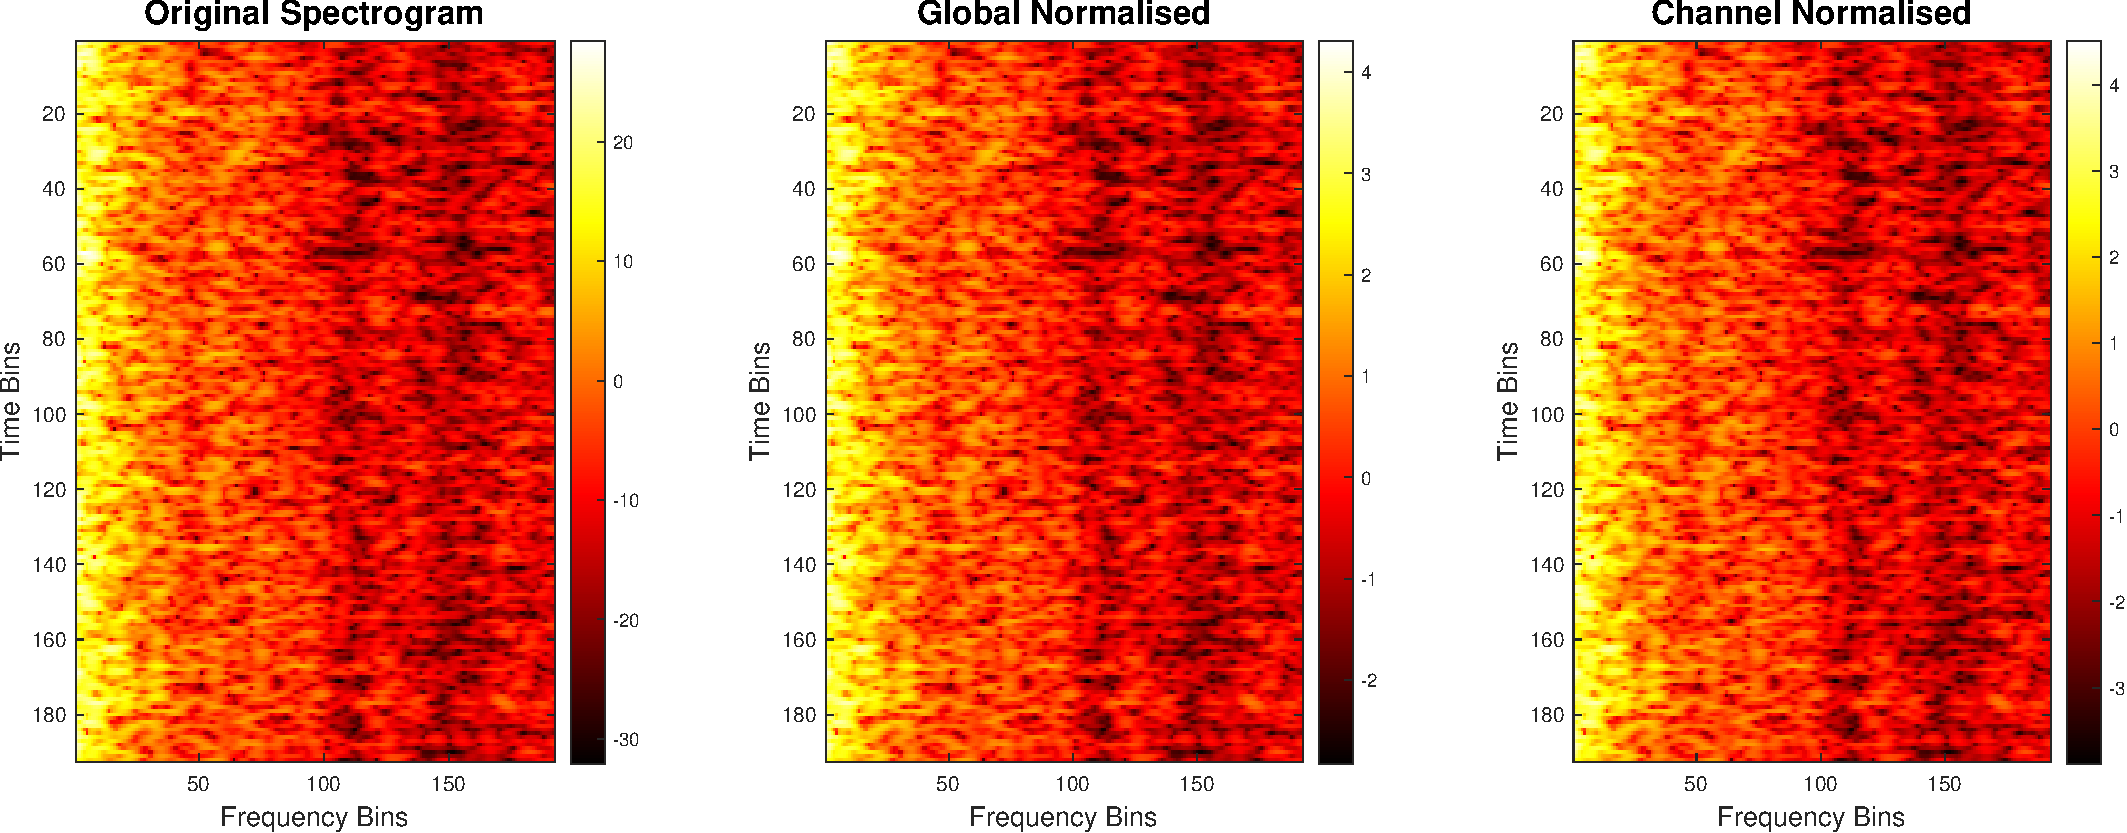
\includegraphics[width=\textwidth]{img/ch4/spectrogramComparison.pdf}
        \caption{Comparison of original spectrogram with global-normalised and channel-normalised spectrograms.}
        \label{fig:normalisation-spectrogram}
    \end{subfigure}
    
    \vspace{1cm}
    
    % Subfigure 2: Histogram Comparison
    \begin{subfigure}[t]{\textwidth}
        \centering
        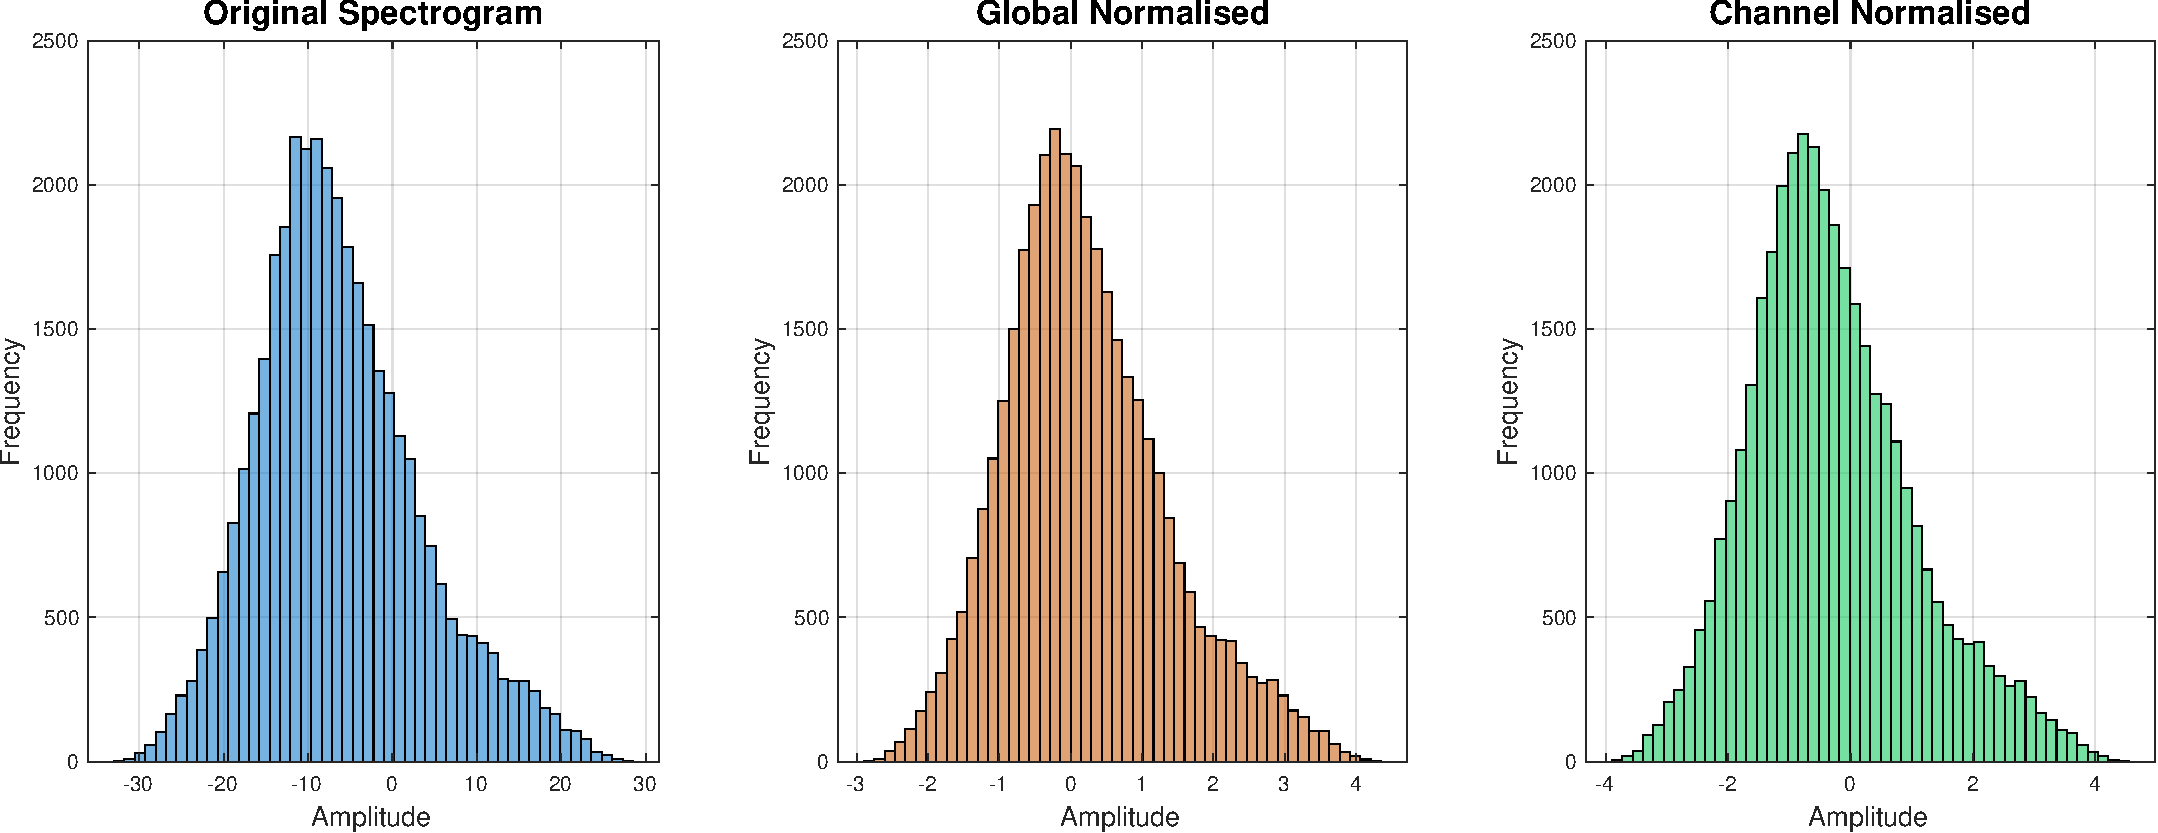
\includegraphics[width=\textwidth]{img/ch4/histogramComparison.pdf}
        \caption{Comparison of amplitude histograms for original, global-normalised, and channel-normalised spectrograms.}
        \label{fig:normalisation-histogram}
    \end{subfigure}
    
    \vspace{1cm}
    
    % Subfigure 3: Time Segment Comparison
    \begin{subfigure}[t]{\textwidth}
        \centering
        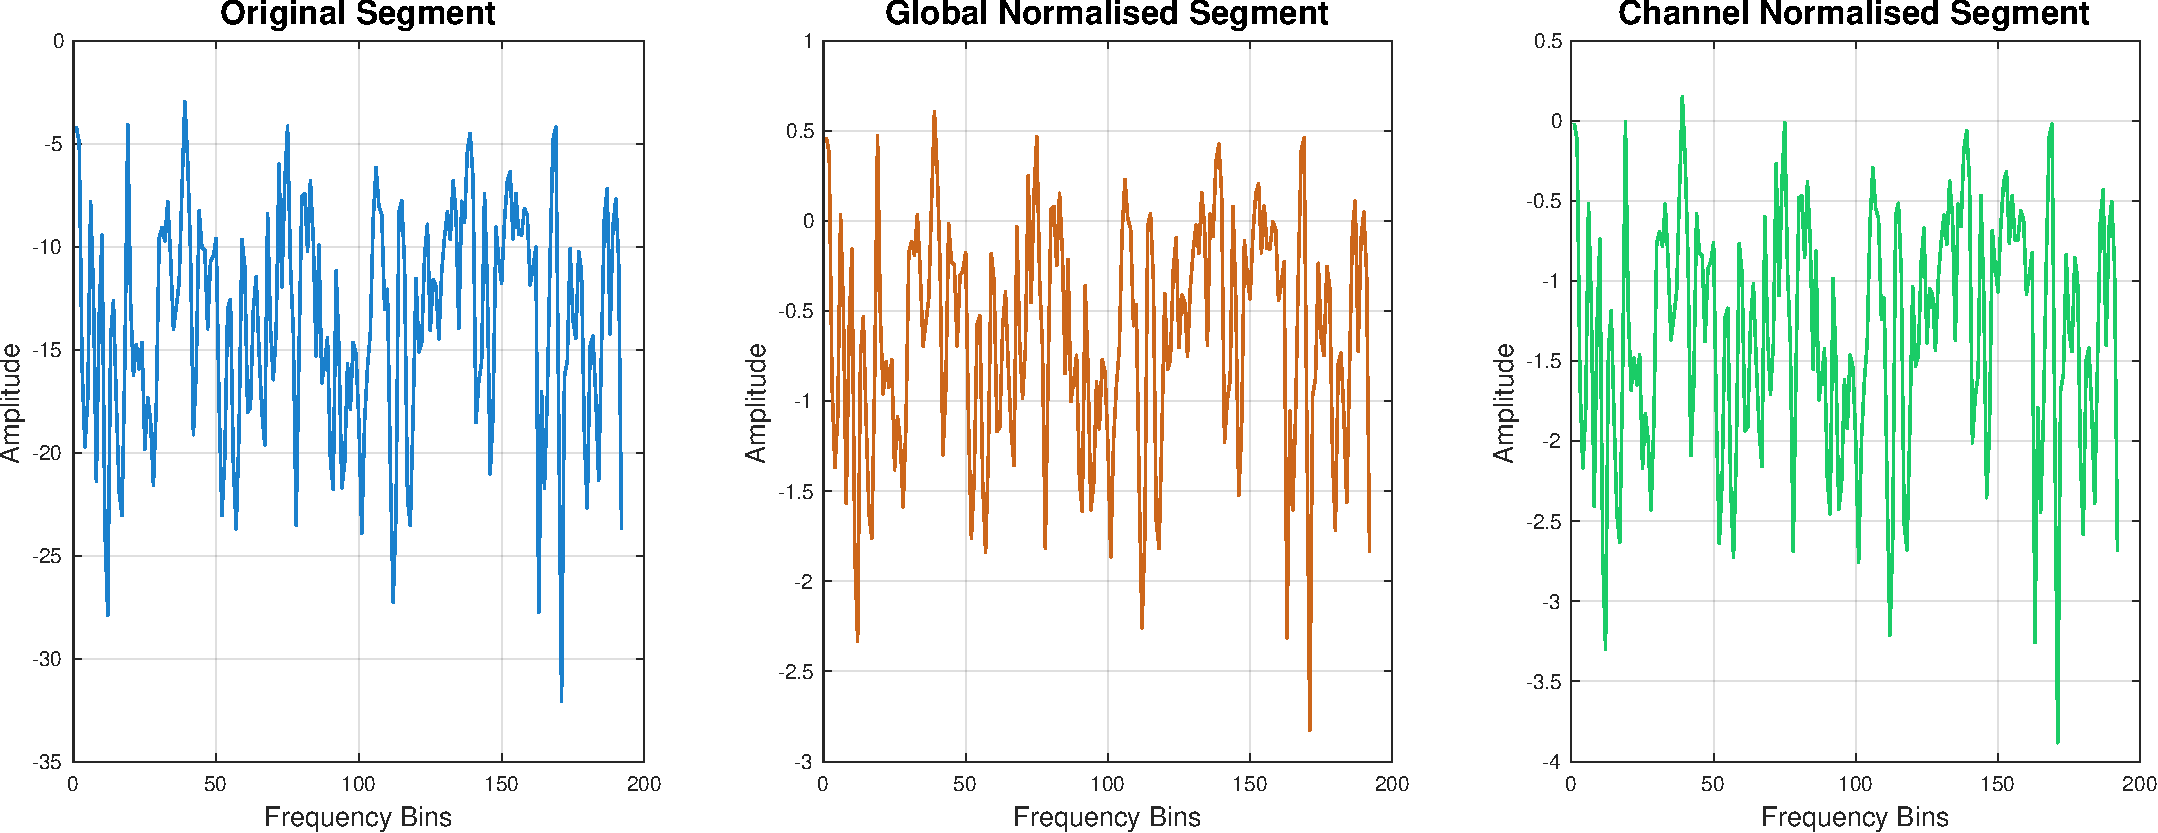
\includegraphics[width=\textwidth]{img/ch4/timeSegmentComparison.pdf}
        \caption{Comparison of a random time segment for original, global-normalised, and channel-normalised spectrograms.}
        \label{fig:normalisation-time-segment}
    \end{subfigure}

    \caption{Visual comparison of normalisation methods.}
    \label{fig:normalisation-combined}
\end{figure}

The comparison of original, global-normalised, and channel-normalised spectrograms, as shown in Figure~\ref{fig:normalisation-combined}, reveals minimal visual differences in the structural patterns across the three techniques. This outcome is expected, as the primary purpose of normalisation is not to alter the fundamental structure of the spectrogram but to rescale their amplitudes into a standardised range. The key difference in Figure~\ref{fig:normalisation-spectrogram} lies in the colour bar scaling: in the original spectrograms, amplitude values span a range of approximately $-30$ to 30 dB, whereas in the global and channel-normalised spectrograms, the values are rescaled to a narrower range, approximately $-3$ to 4 dB. This is further supported by Figure~\ref{fig:normalisation-time-segment} which highlights the rescaling of amplitudes for a single random time segment in each spectrogram. Additionally, the amplitude histograms in Figure~\ref{fig:normalisation-histogram} show that while the overall distribution shapes remain similar, the normalised spectrograms exhibit distributions centred around zero. This comparison highlights a key property of normalisation: the normalised spectrograms still retain the important information necessary for classification while standardising the data for greater gradient stability during machine learning tasks.

\section{Experiments}

\subsection{Methodology}

To evaluate the impact of global and channel-based normalisation on the DeepShip dataset, we designed an experiment to compare the performance of our benchmark CNN-LSTM model across three scenarios: baseline (no normalisation), global normalisation, and channel-based normalisation. The objective was to isolate the influence of these normalisation methods on model accuracy.

The DeepShip dataset was converted into power spectrograms as described in Section~\ref{sec:inputs}. The same 10-fold cross-validation splits were used across all experiments to ensure a consistent and fair comparison. Normalisation was implemented as a two-pass operation in MATLAB. In the first pass, the required statistics for normalisation were computed:
\begin{itemize}
    \item For global normalisation, the mean and standard deviation were calculated across all time-frequency bins in the dataset.
    \item For channel-based normalisation, these statistics were calculated separately for each frequency channel. 
\end{itemize}

In the second pass, these precomputed statistics were used to apply the respective normalisation transformations to each spectrogram. The transformed spectrograms were saved as \texttt{.mat} files in separate directories corresponding to the baseline, global, and channel-based normalisation settings.

The benchmark CNN-LSTM model was trained on the spectrograms processed using each normalisation method under identical conditions. The same architecture, hyperparameters, and training configuration were used for all experiments, as outlined in Table~\ref{tab:cnn-lstm-final-params} and Section~\ref{subsec:training-configuration}. Model performance was evaluated using accuracy as the primary metric, and training and validation loss curves were recorded to analyse convergence trends qualitatively.

To ensure reproducibility and consistency, all experiments were conducted using MATLAB version 2024a and Keras 2.10, with a seeded random number generator and GPU-accelerated training.

\subsection{Results}

The results of this experiment show minimal difference between the three normalisation strategies. The baseline model previously achieved an accuracy of 63.41\%, while both global and channel-based normalisation resulted in lower accuracies of 62.99\% and 63.16\% respectively. The results of these experiments are summarised in Table~\ref{tab:normalisation-results}. Training and validation accuracy-loss curves are shown in Figure \ref{fig:channel-norm-acc-loss} and \ref{fig:global-norm-acc-loss} (Appendix \ref{curves:normalisation}).

\begin{table}[h]
    \centering
    \caption{Comparison of normalisation strategies on the DeepShip dataset.}
    \label{tab:normalisation-results}
    \begin{tabular}{lcc}
        \toprule
        \textbf{Normalisation strategy} & \textbf{Accuracy (\%)} & \textbf{Precision} \\
        \midrule
        Global normalisation            & 62.99 & 65.66 \\
        Channel-based normalisation     & 63.16 & 66.34 \\
        \textbf{Baseline ($\bm{\log_{10}}$)}  & \textbf{63.41} & \textbf{66.53} \\
        \bottomrule
    \end{tabular}
\end{table}

\subsection{Discussion}

This lack of significant improvement was unexpected, particularly given the previous research on the theoretical and practical benefits of normalisation for machine learning tasks (\cite{chris_kroenke_normalizing_2022, gunes_answer_2020, wu_group_2018, primus_frequency-wise_2023, simic_normalization_2023}). One possible explanation lies in the relatively consistent scale and distribution of spectrogram features in the DeepShip dataset, likely due to the logarithmic transformation undertaken to convert the spectrogram into a power spectrogram representation. This transformation inherently normalises the input values, perhaps diminishing the benefit of additional explicit normalisation techniques.

A key limitation of the experiment was the approach taken to calculate the normalisation statistics. In standard practice, the mean and standard deviation are calculated on the training set and then applied to both the training and test sets. This ensures that the test data remains unseen during the calculation of normalisation parameters, preserving the integrity of the evaluation process and preventing data leakage. However, due to the $k$-fold cross-validation setup used in this study, where training and testing sets change dynamically in each fold, it was impractical to calculate the mean and standard deviation exclusively from the training set. Instead, normalisation statistics were computed using the entire dataset, which may have introduced a minor data leakage effect. While this compromise was necessary given the experimental constraints, it could explain the minimal differences observed between the strategies.

Additionally, it is possible that the relatively short training duration of five epochs limited the ability of the model to fully leverage any benefits introduced by normalisation. Normalisation's primary advantages, such as stabilising gradient flow and accelerating convergence, may become more evident over longer training periods or with deeper models.

The training and validation accuracy-loss curves for both the channel normalisation experiment (Figure \ref{fig:channel-norm-acc-loss}) and global normalisation experiment (Figure \ref{fig:global-norm-acc-loss}) show great similarity between not only each other but also the benchmark model's accuracy-loss curves (Figure \ref{fig:baseline-acc-loss}), signifying that the training procedure went well with no errors, but also no great improvements as was previously postulated.

Finally, it is worth noting that while normalisation did not significantly impact classification accuracy, it may still have other advantages not captured in this experiment, such as enabling more efficient training and model convergence. Future work could explore these aspects more thoroughly.

\subsection{Conclusion}

This experiment demonstrated that global and channel-based normalisation had minimal impact on classification performance for the DeepShip dataset, with results obtained comparable to the baseline (unnormalised) model. The minimal improvement suggests that the preprocessing steps already applied -- such as the power spectrogram logarithmic conversion -- played a significant role in standardising the input data, diminishing the additional benefits typically offered by explicit normalisation.

These findings highlight the importance of aligning preprocessing strategies with the specific characteristics of a dataset. Future work could explore alternative normalisation techniques, such as 0-1 normalisation or local normalisation, and examine their effects over longer training cycles or their role in improving training stability and convergence. Additionally, future researchers may wish to begin with amplitude spectrograms rather than power spectrograms to isolate the impact of normalisation without other preprocessing factors influencing the results. Such investigations could provide deeper insights into the role of normalisation in underwater acoustic signal classification.